% !TEX TS-program = pdflatex
% !TEX encoding = UTF-8 Unicode

% This is a simple template for a LaTeX document using the "article" class.
% See "book", "report", "letter" for other types of document.

\documentclass[11pt]{article} % use larger type; default would be 10pt


\usepackage{ulem}
\newcommand\NoIndent[1]{%
  \par\vbox{\parbox[t]{\linewidth}{#1}}%
}


\usepackage[utf8]{inputenc} % set input encoding (not needed with XeLaTeX)

%%% Examples of Article customizations
% These packages are optional, depending whether you want the features they provide.
% See the LaTeX Companion or other references for full information.

%%% PAGE DIMENSIONS
\usepackage{geometry} % to change the page dimensions
\geometry{a4paper} % or letterpaper (US) or a5paper or....
% \geometry{margin=2in} % for example, change the margins to 2 inches all round
% \geometry{landscape} % set up the page for landscape
%   read geometry.pdf for detailed page layout information

\usepackage{graphicx} % support the \includegraphics command and options

% \usepackage[parfill]{parskip} % Activate to begin paragraphs with an empty line rather than an indent

%%% PACKAGES
\usepackage{booktabs} % for much better looking tables
\usepackage{array} % for better arrays (eg matrices) in maths
\usepackage{paralist} % very flexible & customisable lists (eg. enumerate/itemize, etc.)
\usepackage{verbatim} % adds environment for commenting out blocks of text & for better verbatim
\usepackage{subfig} % make it possible to include more than one captioned figure/table in a single float
% These packages are all incorporated in the memoir class to one degree or another...

%%% HEADERS & FOOTERS
\usepackage{fancyhdr} % This should be set AFTER setting up the page geometry
\pagestyle{fancy} % options: empty , plain , fancy
\renewcommand{\headrulewidth}{0pt} % customise the layout...
\lhead{}\chead{}\rhead{}
\lfoot{}\cfoot{\thepage}\rfoot{}

%%% SECTION TITLE APPEARANCE
\usepackage{sectsty}
\allsectionsfont{\sffamily\mdseries\upshape} % (See the fntguide.pdf for font help)
% (This matches ConTeXt defaults)

%%% ToC (table of contents) APPEARANCE
\usepackage[nottoc,notlof,notlot]{tocbibind} % Put the bibliography in the ToC
\usepackage[titles,subfigure]{tocloft} % Alter the style of the Table of Contents
\renewcommand{\cftsecfont}{\rmfamily\mdseries\upshape}
\renewcommand{\cftsecpagefont}{\rmfamily\mdseries\upshape} % No bold!

%%% END Article customizations


\usepackage{verbatim}
\usepackage{amsmath}






\title{Work Log for September}
\author{Logan Brown}
%\date{} % Activate to display a given date or no date (if empty),
         % otherwise the current date is printed 

\begin{document}
\maketitle
%\tableofcontents


\setcounter{section}{2} %week number minus 1
\setcounter{subsection}{-1}
\setcounter{subsubsection}{0}

\section{Week of September 15th-19th}
\subsection{Goals for the Week}
%Paste output from writeGoals
\begin{enumerate}
\item Simulated Data Set
\item First Order Approximation
\item Potentially look at the c files in cubfits/cubfits/src
\item Check for problems in Wei-Chen's NSE code, specifically, a crash caused by running out of memory
\item Continue to improve the optimal-pessimal code as Deepika works with it.

\end{enumerate}

\subsection{Progress/Notes}

\subsubsection{Simulated Data Set}
The data is in /home/lbrown/reucode/data/inputsimdata/REU\_data

As I understand it, these fasta genomes are ones that have been modified by Codon Evolution Simulation (CES). A quick comparison of  b-1/S.cerevisiae.S288c.REU.sim.b-1.ces.fasta and ../S.cerevisiae.S288c.fasta shows that they have different codons. Additionally b-1's fasta file and b-0.01's fasta are different as well.

The folder b-1 vs b-0.1, etc is the setting of the B parameter. Look at '/export/home/clandere/CodonUsageBias/NSE/ces3/branches/exchange/C/data\_simulation/CES.DATA.SIM.README.pdf' for more details

I chose to use b-0.001, it had the best signs of actually converging to something. The eta values of the genes actually changed. For some b values, there wasn't an eta change. b-0.001/S.cerevisiae.S288c.REU.sim.b-0.001.evol.summary.tsv was the highest B value that had changes at every genome (Evolution Time != nan). 

I was not able to find X\_obs values for the yeast data in the REU data. I found ORF data in /opt/big\_scratch/work-my, which is data from Wei-Chen/Yassour. I ran a recursive search through those files looking for xobs values, the output is found in smallfindXobs.txt



\subsubsection{cubappr SimuYeast Run}
Launched a cubappr run of the simulated yeast genome from the REU data, both for single chain and \sout{multichain} (nothing happened for ~2 hours. either it crashed, or changing the config.r file messed with the actual inner workings). If either/both crashes, I'll try again with a smaller run, likely just singlechain.


\subsubsection{First Order Approximation}

$$\prod_{j=i+1}^{n} (1-p_j)= \prod_{j=i+2}^{n} - p_{i+1}\left(\prod_{j=i+2}^{n}(1-p_{i+1})\right)$$

Simply to make things easier to read, I'll restate $\prod_{j=q}^{n} (1-p_j)$ as $t_q$. Note that in general,

$$t_q = t_{q+1} - p_q(t_{q+1})$$

So 

\begin{align*}
	\prod_{j=i+1}^{n} (1-p_j) &= t_{i+2} - p_{i+1}t_{i+2} \\
	&= t_{i+3} - p_{i+2}t_{i+3} - p_{i+1}\left(t_{i+3} - p_{i+2}t_{i+3}\right) \\
	&= t_{i+3} - p_{i+2}t_{i+3} - p_{i+1}t_{i+3} - p_{i+1}p_{i+2}t_{i+3}
\end{align*}

Since $p_{i+1} * p_{i+2} \approx 0$.

$$\approx t_{i+3} - p_{i+2}t_{i+3} - p_{i+1}t_{i+3}$$

Continuing iteratively...

\begin{align*}
	\prod_{j=i+1}^{n} (1-p_j) &\approx
	t_n - \sum_{k=i+1}^{n-1}p_k(t_n) \\
	&\approx (1-p_n) - \sum_{k=i+1}^{n-1}p_k(1 - p_n)\\
 	&\approx 1 -  \sum_{k=i+1}^{n}p_k
\end{align*}

\subsubsection{Potentially look at the c files in cubfits/cubfits/src}
They still look like they aren't doing anything.

\subsubsection{Investigate WeiChen NSE crash}
\begin{itemize}
\item Ending crash caused by running out of memory?
\end{itemize}

Cedric also suggests it could be due to a problem with the serialization step. When the code is run in parallel (by SNOW activating multiple copies of the same program with different initial conditions), it comes back to the serial to be tested for convergence. If the data structures are too large at this point, it may crash due to "running out of memory", even though Gauley has waaay more memory. It may be related to memory.c

I'm running in single chain from here on out for testing this hypothesis.

Single chain crashed, however, it actually told the error!

\verbatiminput{data/sep15.SimYeastNSE.error.txt}

\subsubsection{Compare NSE code to ROC code}

Here are all the files that use the NSE model (results of grep -il nse ~/cubfits/cubfits/R/*)


\sout{my.coef.r}\\

my.estimatePhiOne.r\\
my.fitMultinomOne.r

Here is where the vglm concerns are. Mostly not concerned, it doesn't look like any additional vglm calls.\\


my.logdmultinomCodOne.r\\

Here's my biggest concern. 


my.logdmultinomCodOne.roc has three lines that my.logdmultinomCodOne.nsef does not
  lp.c.raw <- yaa * lp.vec
  lp.c.raw[is.nan(lp.c.raw)] <- NA
  lp.c.raw <- rowSums(yaa * lp.vec, na.rm = TRUE)

my.drawPhiConditionalAllPred calls my.logPosteriorAllPred.lognormal, which calls my.logdmultinomCodOne.nsef, which does not have the stated lines. Without those lines, if lpProp - lpCurr - prop\$lir becomes NaN (log of a negative value, most likely), it would not pass any errors until the line that actually complains, accept <- u < exp(logAcceptProb).

However logAcceptProb is lpProp - lpCurr - prop\$lir

My best hypothesis is that lpProp (proposed phi values from the Posterior distribution) has some NaN values.




my.objectivePhiOne.Lfp.r\\
my.objectivePhiOne.nlogL.r\\
my.objectivePhiOne.nlogphiL.r\\
my.objectivePhiOne.phiLfp.r\\
my.pPropTypeNoObs.lognormal\_bias.r\\
plotbin.r\\
plotmodel.r\\
simu.orf.r\\


\subsubsection{Build Local Cubfits}

\begin{enumerate}
\item cd path/to/cubfits/..
\item R CMD build cubfits (This creates cubfits\_ver.si-on.tar.gz)
\item R
\item install.package("\_\_\_\_\_\_\_.tar.gz", lib ="place to install to", repos = NULL, type="source")
\item library(cubfits, lib.loc="place you installed to")
\end{enumerate}


\subsubsection{Disect NSE data Structure}

\subsubsection{Profile the ROC model (where is the time?)}
Look at the man page - ?Rprof 

%Rprof(filename = "Rprof.out", memory.profiling = TRUE);
Run Rprof() before any code you want to profile, and Rprof(NULL) after the code, then run summaryRprof in R or R CMD Rprof from the command line to analyze the output. 

Added Rprof() to the beginning of run\_roc.r and Rprof(NULL) to the end of run\_roc.r, then ran using ./workflow as usual.

These are the functions that took up more than 1\% of the time on their own.
\verbatiminput{data/ROCprofile1percent}

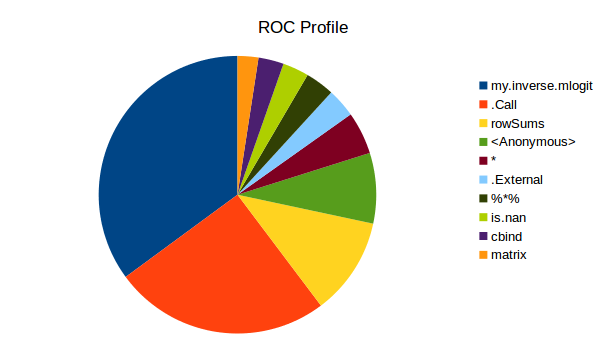
\includegraphics{data/ROCprofile}
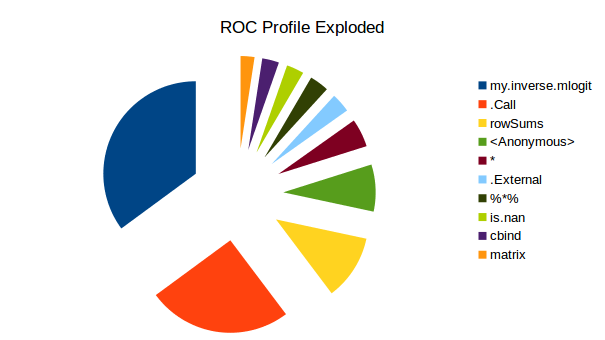
\includegraphics{data/ROCprofilexplode}

.Call is only seen in the 



\subsubsection{Continue to improve the optimal-pessimal code as Deepika works with it.}





\subsection{Goals for next Week}
\begin{enumerate}
\item Future Goal
\end{enumerate}


\end{document} %End of day document, REMOVE
